\section{Image Descriptor}

For the implementation of the clustering we consider OpenCV implementation of K-means, and for the connected components we implemented a Bread-First Search, the results for clustering are shown in figure \ref{fig:clusters}. We apply a median filter before the clusting in order to remove noise while preserving edges. Experiments whit diferents number of clusters $K$ are computed ($K = 2, 4, 8$).

\begin{figure}[!h]
	\centering
	\begin{subfigure}{0.5\textwidth}
	  \centering
	  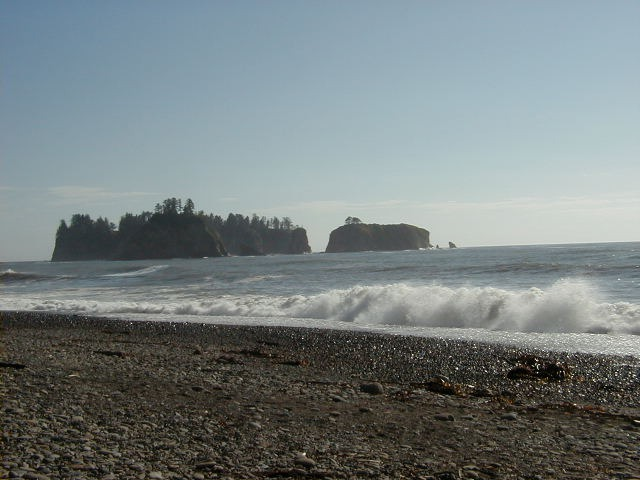
\includegraphics[width=0.9\linewidth]{figs/beach_1.jpg}
	  \caption{Original Image}
	\end{subfigure}%
	\begin{subfigure}{0.5\textwidth}
	  \centering
	  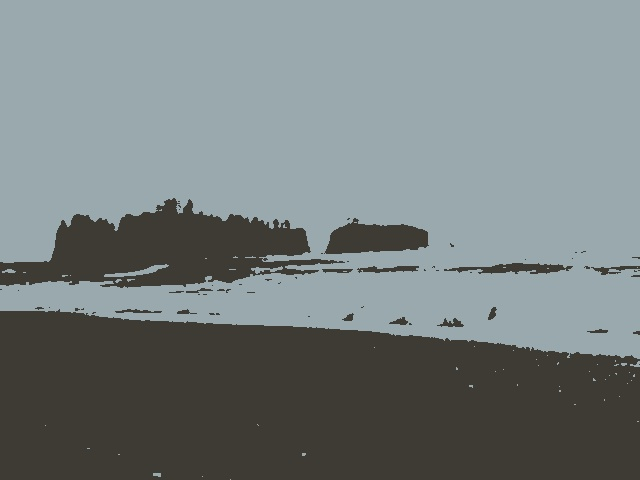
\includegraphics[width=0.9\linewidth]{figs/beach_1_clustK2.jpg}
	  \caption{$K$ = 2}
	\end{subfigure}
	\begin{subfigure}{0.5\textwidth}
        \centering
        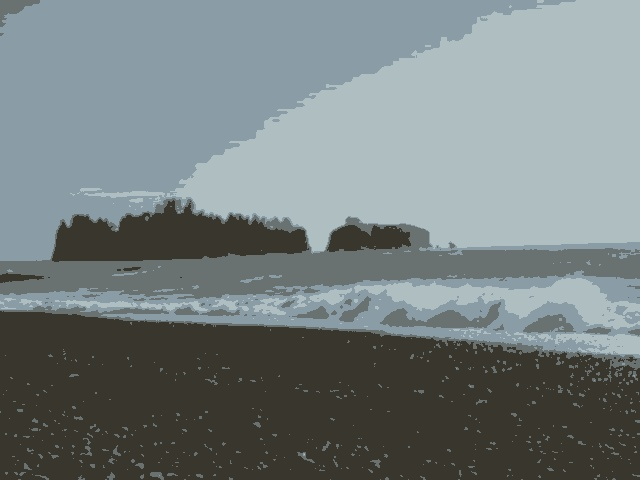
\includegraphics[width=0.9\linewidth]{figs/beach_1_clustK4.jpg}
        \caption{$K$ = 4}
    \end{subfigure}%
    \begin{subfigure}{0.5\textwidth}
	  \centering
	  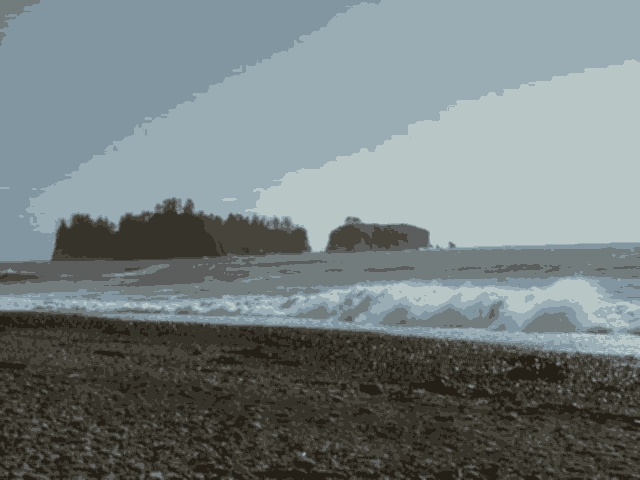
\includegraphics[width=0.9\linewidth]{figs/beach_1_clustK8.jpg}
	\caption{$K$ = 8}
	\end{subfigure}
	
    \caption{Comparison of clustering results for differentes values of $K$}
	\label{fig:clusters}
\end{figure}

Comparing the results of figure \ref{fig:clusters}, with a low number of clusters, the scence losses its essence, while with a bigger number its look more natural and is similar to the origin one.

The results for the conected components are shown in figure \ref{fig:components}, note that there are black areas, this is because components with less than $threshold$ pixels are not consider in further steps. We consider experiments with differents values of $threshold$ ($threshold = 100, 300 $).

\begin{figure}[H]
	\centering
	\begin{subfigure}{0.5\textwidth}
	  \centering
	  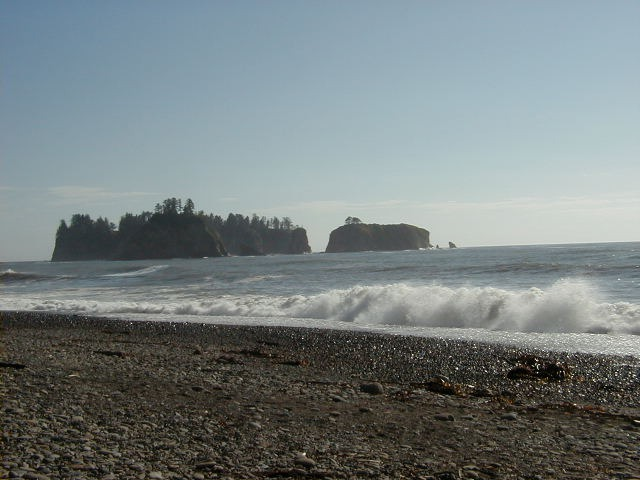
\includegraphics[width=0.9\linewidth]{figs/beach_1.jpg}
	  \caption{Original Image}
	\end{subfigure}%
	\begin{subfigure}{0.5\textwidth}
	  \centering
	  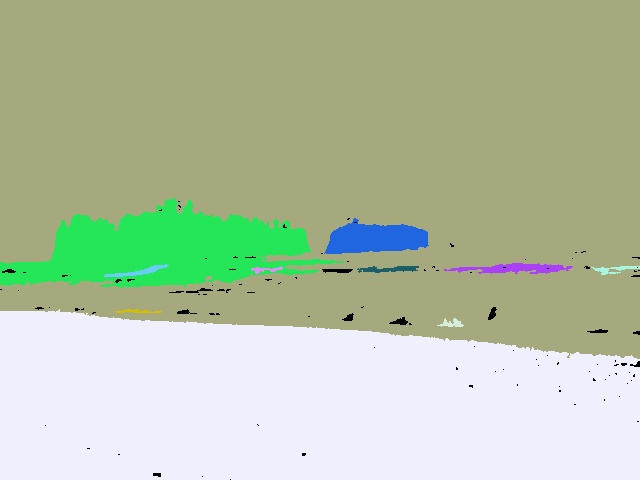
\includegraphics[width=0.9\linewidth]{figs/beach_1_compK2.jpg}
	  \caption{$K$ = 2}
	\end{subfigure}
	\begin{subfigure}{0.5\textwidth}
        \centering
        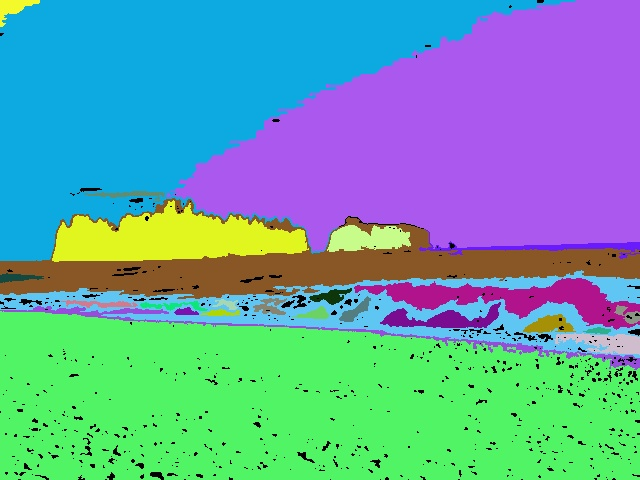
\includegraphics[width=0.9\linewidth]{figs/beach_1_compK4.jpg}
        \caption{$K$ = 4}
    \end{subfigure}%
    \begin{subfigure}{0.5\textwidth}
	  \centering
	  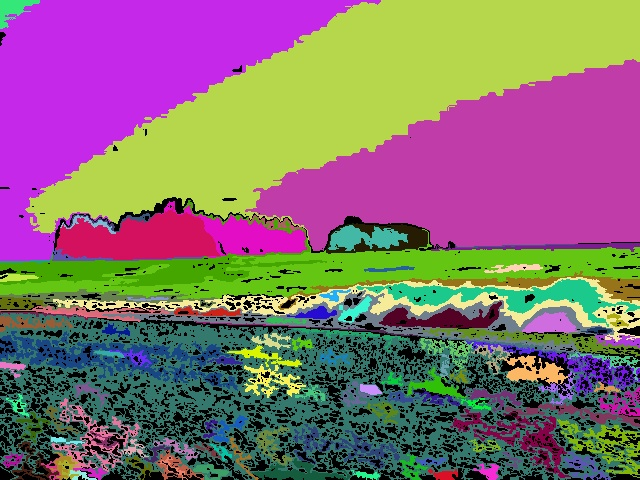
\includegraphics[width=0.9\linewidth]{figs/beach_1_compK8.jpg}
	\caption{$K$ = 8}
	\end{subfigure}
	
    \caption{Comparison of conected components results for differentes values of $K$}
	\label{fig:components}
\end{figure}

From figure \ref{fig:components} we can see that the number of clusters has big impact in the components, note that in the case of $K= 8$ there are various areas with small size, that is why we consider a $threshold$ in the size of each component.

In order to describe the image we consider:

\begin{itemize}
\item \textbf{Size of region}: The number of pixels of each component is considered as the size of the region.
\item \textbf{Mean color}: The mean color was calculated indendly for each channel.
\item \textbf{Contrast}: This metric was computed from the gray co-ocurrence matrix, we use \textit{scikit-image} implementation of this function.
\item \textbf{Correlation}: This metric was computed from the gray co-ocurrence matrix, we use \textit{scikit-image} implementation of this function.
\item \textbf{Entropy}: This metric was computed from the gray co-ocurrence matrix given by \textit{scikit-image}, we implemented this function from the scratch.
\item \textbf{Centroid of the region}: We consider the concept of moments to compute this feature.
\item \textbf{Bounding box}: We consider as bounding box, the quadrilateral that envolves the component, with its sides parallel to image sides, and the feature is the size of the diagonal of this bounding box.
\end{itemize}

In section \ref{sec:experiments} we compare different combinations of these features.

